\section{Hydraulic Erosion Using Smoothed Particle Hydrodynamics}
In this publication \cite{krivstof2009hydraulic} a novel approach is presented, in which a physically based erosion system can be calculated in real-time. The Base concepts are quite the same as in the previously mentioned publication, but as the title reveals the already know SPH is used as underlining base model here.

\begin{figure}[htb]
	\centering
	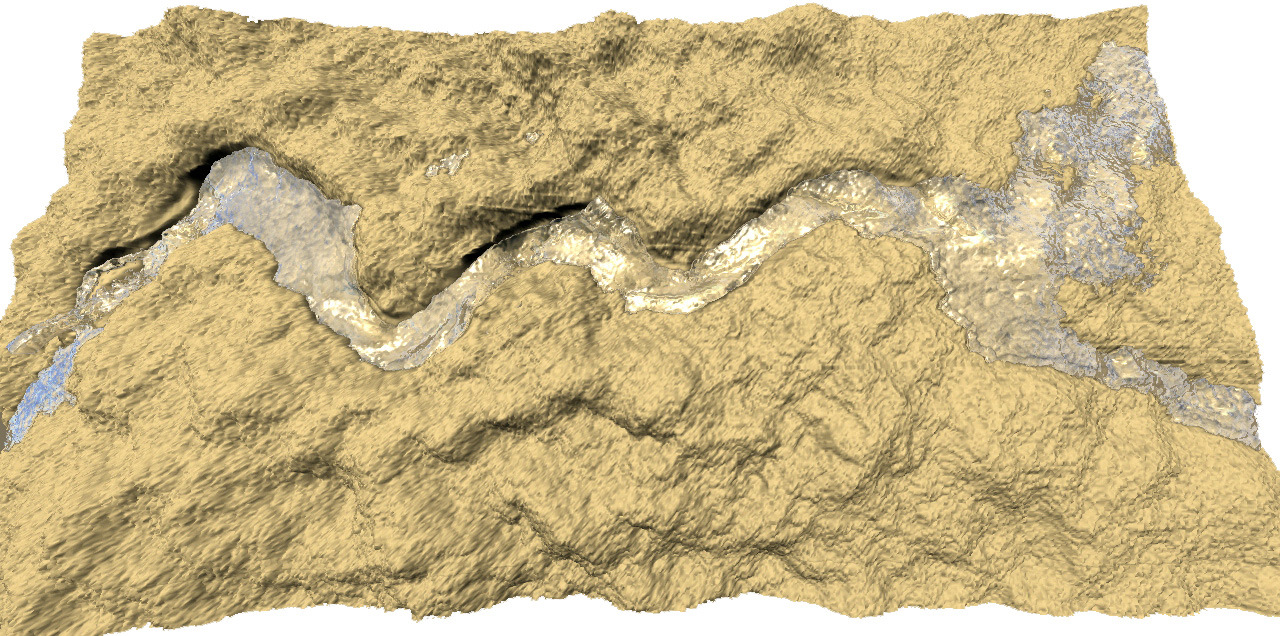
\includegraphics[width=\linewidth]{KBKS09/illustration1.jpg}
	\caption{Rendering of the path of a river in soil.}
	\label{fig:illustration1}
\end{figure}


\begin{figure}[htb]
	\centering
	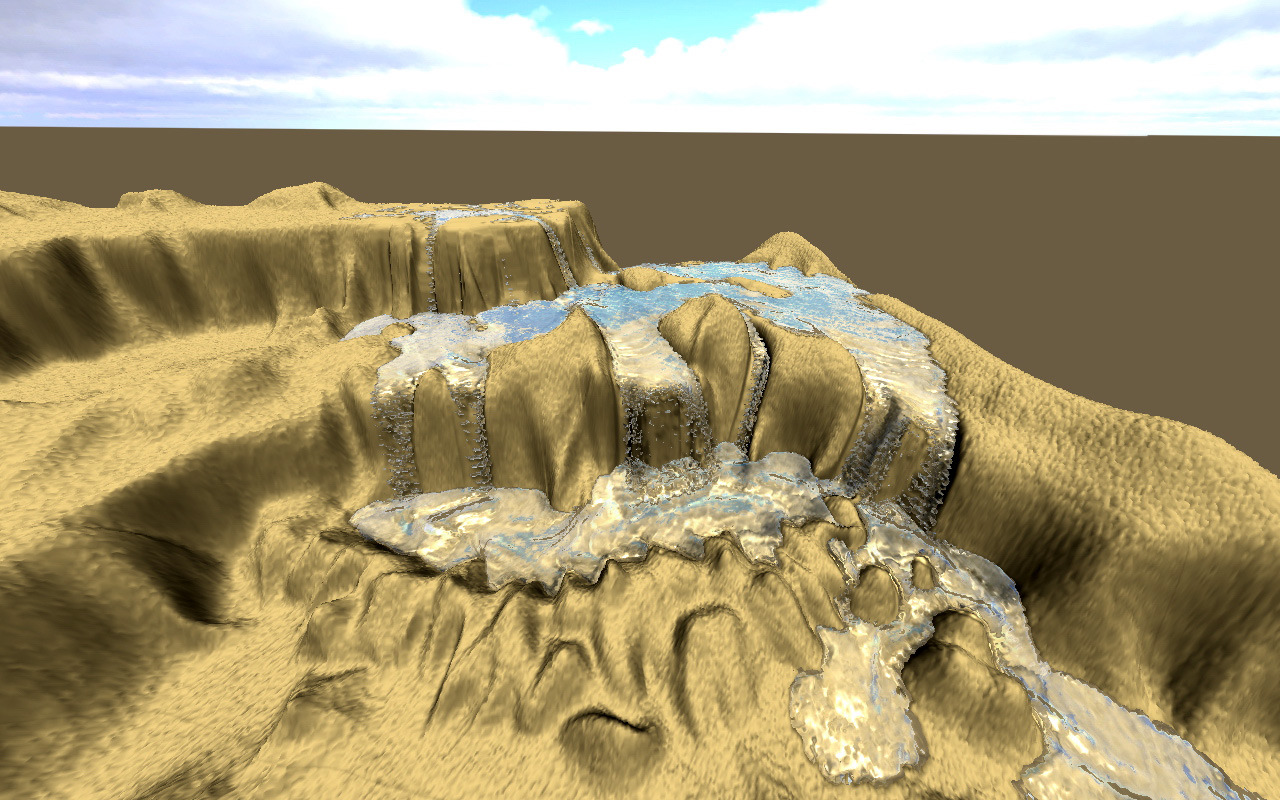
\includegraphics[width=\linewidth]{KBKS09/illustration2.jpg}
	\caption{Rendering of terrain erosion through water.}
	\label{fig:illustration2}
\end{figure}

\subsection{Two different approaches}
An important distinction is made between two different calculation approaches:

\subsubsection{The Eulerian model}
The Eulerian models focuses on hydraulic erosion effects and therefore use a static grid of points. A full scale 3D calculation on approach for erosion calculation is almost impossible to be done in real-time. Most used methods therefore rely on "2.5D" methods, which combine purely surface- / plane-based models with parts of a full 3D approach.

\subsubsection{The Lagrangian model}
Lagrangian models are based on SPH and calculate their results on particle basis. Due to that fact, these methods are much more scalable. Since everything is calculated on particle basis, this approach yields better more exact results in areas, with a high density of particles.

Since there are a lot of necessary calculations to be done which increase linearly with the number of particles, a purely 3D calculation model is rarely used here. As with the Eulerian approach, a combination of calculations on 2D and 3D basis is used. Although this method was not exactly designed with real-time rendering in mind, the resulting "2.5D" approach yields relatively good results while still remaining reducing the time needed to the calculations drastically.

Since in SPH based approaches all calculations are particle-based, many physical (side-)effects can quite easily be implemented. The basic sediment transport can be calculated using widely known formulas \cite{krivstof2009hydraulic}. In addition to that, a Donor-Acceptor scheme (see Figure \ref{fig:donoracceptor}) is used here, which takes interaction between particles along their velocity, as well as gravity into account \cite{krivstof2009hydraulic}.

\begin{figure}[htb]
	\centering
	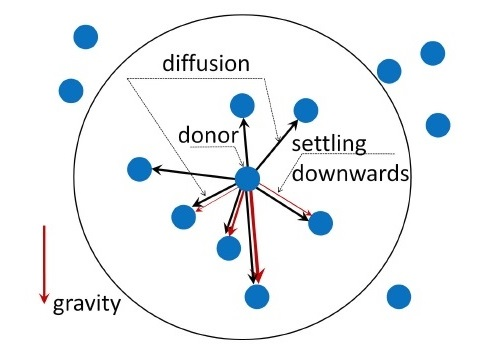
\includegraphics[width=\linewidth]{KBKS09/donoracceptor.jpg}
	\caption{The Donor-Acceptor Scheme.}
	\label{fig:donoracceptor}
\end{figure}

An important concept here are the so called "boundary particles", which also play an important role in the aspect of Terrain Modification as it can be seen in Figure \ref{fig:illustration1} and \ref{fig:illustration2}. Those particles basically are the "communication" between the fluid particles (SPH) and the soil where the boundary particles are placed. In the first iteration the erosion and deposition are calculated, and in the second step / iteration the actual deformation of the terrain itself is performed (see Figure \ref{fig:boundary2}). 

\begin{figure}[htb]
	\centering
	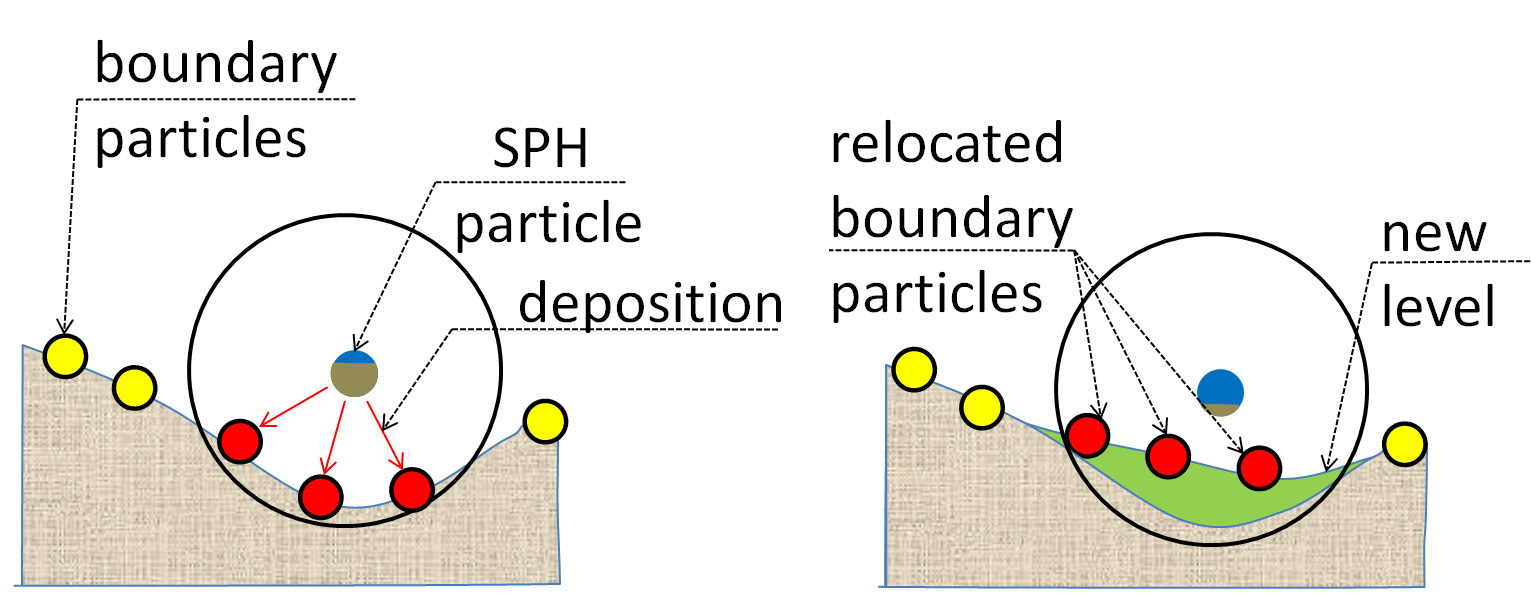
\includegraphics[width=\linewidth]{KBKS09/boundary2.jpg}
	\caption{SPH boundary particle relocation.}
	\label{fig:boundary2}
\end{figure}

\subsection{Performance}
Since this approach was, as mentioned before, not designed with any real-time applications in mind, the underlying publication does not provide us with comparable frame times. The authors, however, do present measures for single calculation step  for a certain amount of particles for each discussed method.

It has to be kept in mind that those numbers represent just the time needed for the actual calculation. Therefore they can not simply be converted to frames-per-second since there would of cause be some overhead in computing the actual visualisation in addition to the calculations of the underlying model itself. But for the sake of comparison, we did translate those numbers into rough fps-estimations which can easily be done by taking the reciprocal value of the needed time in seconds needed. In doing so, we quickly realize that this approach is (at least with the used hardware) far from real-time capable.

The utilized hardware was quite common at that time (2008): a Quad Core CPU and a NVIDIA 8800 GT. The average frames per seconds are about 3.3 for 90k particles and around 2.2 for 136k particles. The specific hardware components and complete results can be found in \cite{krivstof2009hydraulic}.



